%%%%%latex preamble%%%%%
\documentclass[titlepage]{article}
%% maxwidth is the original width if it is less than linewidth
%% otherwise use linewidth (to make sure the graphics do not exceed the margin)
\makeatletter
\def\maxwidth{ %
  \ifdim\Gin@nat@width>\linewidth
  \linewidth
  \else
  \Gin@nat@width
  \fi
}
\makeatother

\usepackage[]{color}
\usepackage{rotating}
\usepackage{listings}
\usepackage{alltt}
\usepackage[sc]{mathpazo}
\usepackage{amsmath, amsthm, amssymb}
\usepackage{graphicx}
\usepackage[T1]{fontenc}
\usepackage{geometry}
\geometry{verbose,tmargin=2.5cm,bmargin=2.5cm,lmargin=1.5cm,rmargin=1.5cm}
\setcounter{secnumdepth}{2}
\setcounter{tocdepth}{2}
\usepackage{float}
\usepackage{bm}
\usepackage{tikz}
\usetikzlibrary{arrows,automata}
% \usepackage{minted}

 %changes default sectioning commands -> 1,a, etc.
%\usepackage{breakurl}
\renewcommand{\thesubsection}{(\alph{subsection})}
\renewcommand{\thesubsubsection}{\roman{subsection}.}

\usepackage{url}
\usepackage{hyperref}
\hypersetup{pdfborder = {0 0 0}}

%%% Header and Footer %%% 
\usepackage{lastpage}
\usepackage{fancyhdr}
%%% fancy pages for all non-title and chapter heading pages
\pagestyle{fancy}
%%% puts a line in the footer
\renewcommand{\footrulewidth}{0.4pt}
%%% adds a reference to the last page to give a running page count
\fancyfoot[R]{\thepage \ of \pageref{LastPage}} %requires lastpage
%%%% adds author name to bottom left
\fancyfoot[L]{\textit{Aaron Gonzales}}
%%% empty center footer
\fancyfoot[C]{}

%%% Adds class name to left header
\fancyhead[L]{\textit{Machine Learning}}
%%% Adds document name to right header
\fancyhead[R]{\textit{Project 4 Report}}

\IfFileExists{upquote.sty}{\usepackage{upquote}}{}

\begin{document}

\title{Project 4 Report}
\author{Aaron Gonzales}
\maketitle

%%%%%%%%%%%%%%%%%%%%%%%%%%%%%%%%%%%%%%%%%%%%%%%%

\section{Metadata}

\subsection{Team Name: we\_are\_not\_scientists}
Teammates:
\begin{itemize}
    \item Aaron Gonzales
    \item Andres Ruiz
    \item Mike Wyatt
    \item Adam Delora
    \item Jayson Grace
    \item Geoff Alexander
\end{itemize}

Score:
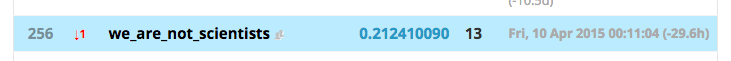
\includegraphics[scale=0.5]{./score.png}
\newpage
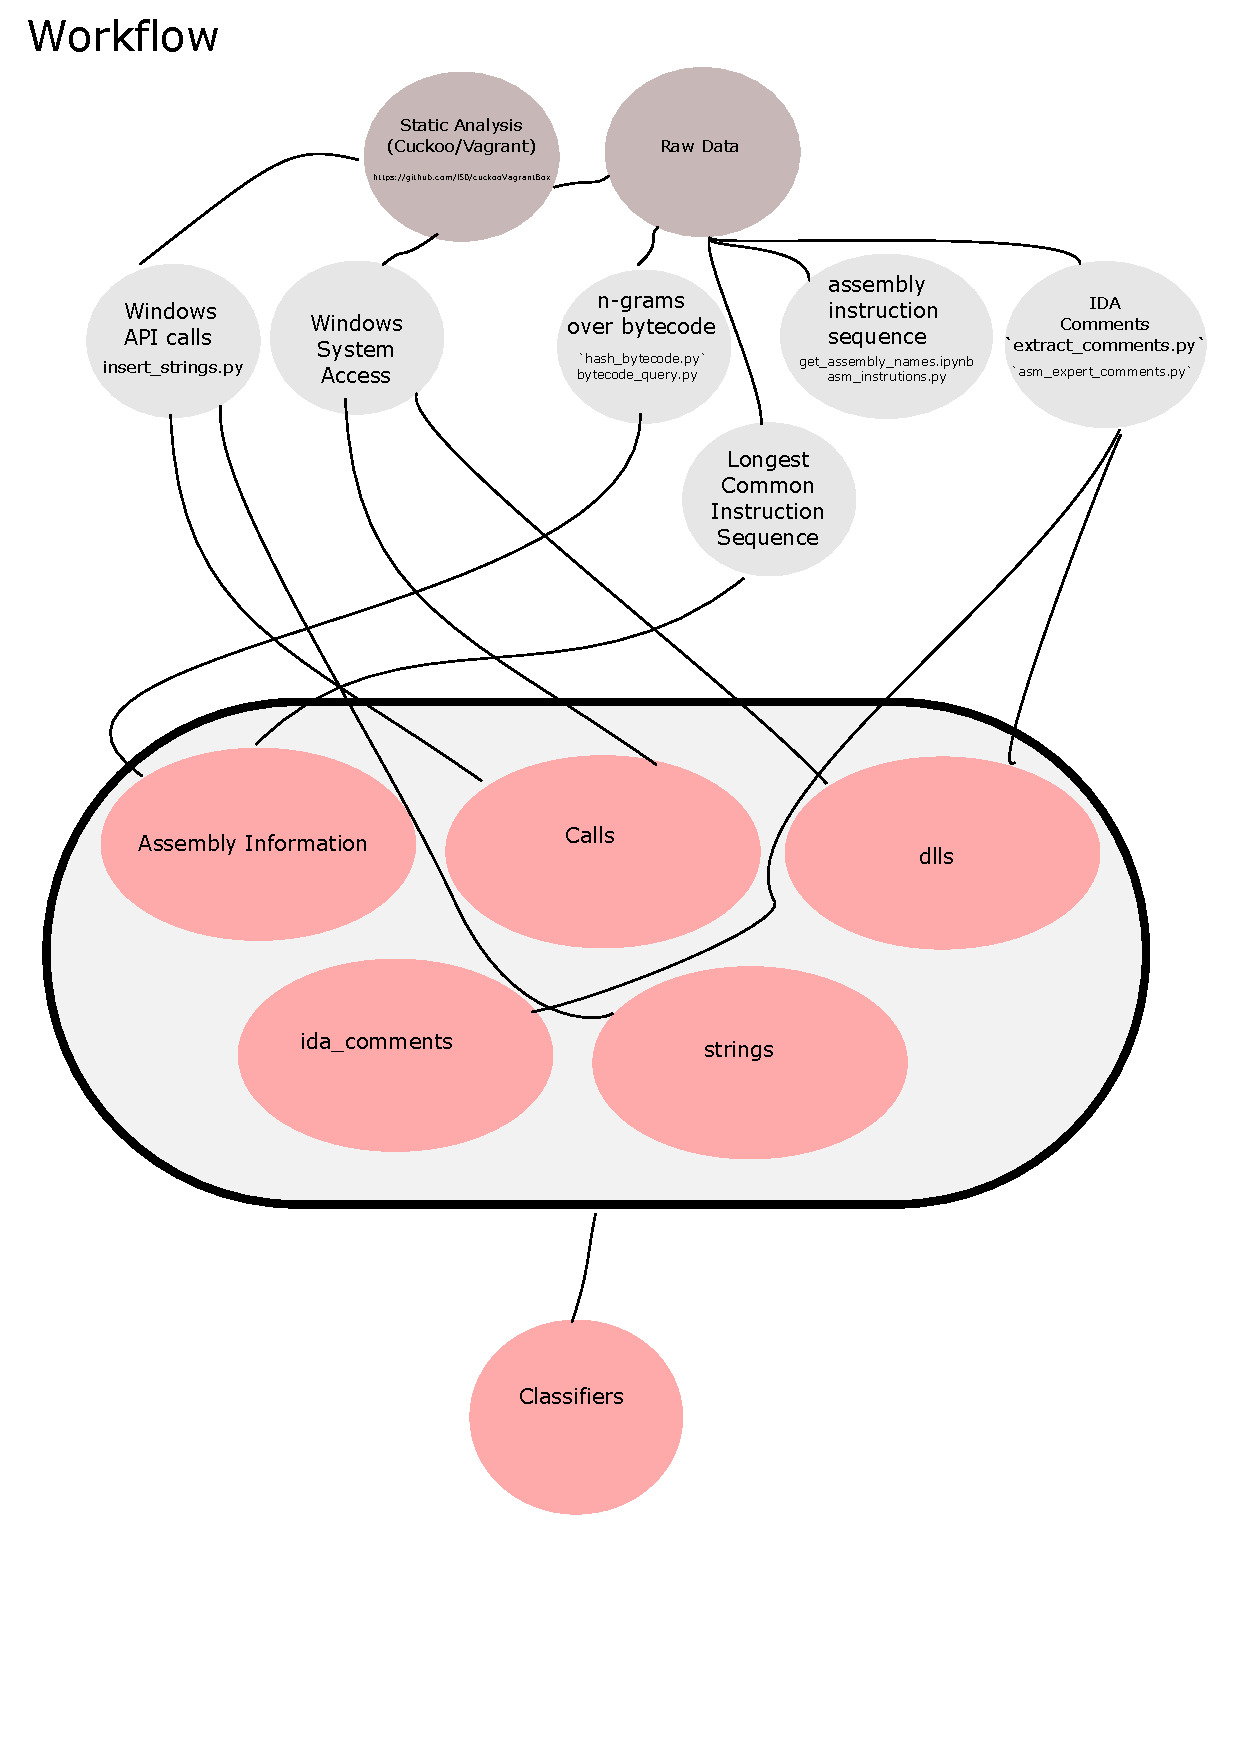
\includegraphics[scale=0.8]{./figure.pdf}

\newpage

\section{Methods used}

\subsection{feature engineering and extraction}
\subsubsection{Summary}
We focused heavily on generating features for our classifiers. Those features
were broken down into several broad categories, relating to information about
the assembly code itself, any files or function calls the program made during
runtime, the comments that the disassembler made, and results from a secondary
dynamic analysis performed by Geoff. Malware can be analyzed statically or
dynamically, where static analysis represents more structure or summary
information about the program and dynamic analysis is where you watch what a
program does under execution in a safe environment and record the outcome.

All data was stored in a centralized MongoDB (NoSQL) database to which every
team member had access.

\subsubsection{Methods used:}

\subsubsection{Dynamic Analysis}
Geoff and Jayson set up environments to analyze the malware's behavior, which
is mostly hosted in Jayson's github repository at
\url{https://github.com/l50/cuckooVagrantBo}. Some of this data was spit out in JSON
format, which was fed directly to Mongo, and some of it required further
processing (Windows API calls / insert\_strings.py).

\subsubsection{Windows API calls}
Geoff did not upload this code to the repository, but it consisted of a
semi-dynamic analysis of malware samples and gave us the dynamically-linked
libraries and windows API function calls accessed by a piece of malware. The
output from this program was very dirty, so a good deal of parsing had to be
done. Aaron built a scraper to get the proper list of function names from
Microsoft's website and used that to help extract some of the names correctly
(and in another area of the project).

\subsubsection{Cuckoo}
Jayson built the analysis pipeline for running a more complete dynamic
analysis. This code lives in the repo mentioned above. Data was organized in
batches to run on several machines, as there were 10,000 samples and each
sample took 90-240 seconds to run.

\subsubsection{n-grams over bytecode}
Following a suggestion on Kaggle, Aaron built methods to extract uni and
bigrams from valid hexidecimal representation of the "raw" bytecode and to
build a bag-of-words model from there, as Scikit-Learn's dict\_vectorizer
didn't handle the data well. The code for these things lives mostly in
bytecode\_query.py. 

\subsubsection{assembly instruction sequence}
This was parsed out from the raw files as a starting point for further feature
engineering. A list of x86 assembly instructions was parsed from the web and
matched against lines in the file. The raw instruction sets were very messy and
difficult to parse without doing this, though it didn't take all that long to
do. The relevant files are get\_assembly\_names.ipynb and asm\_instrutions.py.
Long n-grams (3-8) were generated over this sequence to look for common
patterns (loops) within the code across families, which became a reasonable
feature on its own later.

\subsubsection{Longest common instruction sequence}
Andres built methods to extract the longest common instruction subsequence between all
pairs of files, but this didn't work out due to the computation time involved
(10,000 sequences, 200-500 instructions per sequence, compared to many other
sequences in a class. It was mostly wishful thinking and we moved on to more
cohesive ideas).

\subsubsection{Ida comments}
IDA is the Interactive Dissembler that the malware community uses to generate
human-readable code. It can give valuable annotations in the generated files
and we parsed out the comments to use them as a text feature. This was a tip
from a Mandiant employee. The relevant files are extract\_comments.py and
asm\_expert\_comments.py.

\subsubsection{Assembly statistics}
Our security people recommended doing frequency counts over various types of
actions, which were computed and stored as a set of data within the assembly
code. This included types and numbers of system calls and their subtypes.


\subsection{Classifiers}

\subsubsection{Random Forests}
We had strong cross validation scores (or so we thought; they never broke into
the top scores when submitted to the leaderboard but would achieve roughly
85-92\% cross validated accuracy). Mike mainly ran initial models with these and
did some parameter sweeps over them to eek out more accuracy from the RFs. 

\subsubsection{SVM}
SVMs were ran over several of the text representations (TFIDF over long ngrams,
IDA comments, etc.). Reasonable accuracy was obtained, but again, nothing great
compared to the leaderboard. An SVM with the bytecode uni and bigrams reached
97\% CV accuracy but overfit heavily on the leaderboard score.


\section{What we could have done}
We had several glaring issues with our project. First, as this was purely
extracurricular, not everyone devoted much time to it and several teammates
dropped out before too long (or didn't contribute all that much for various
reasons). As such, most of the work specified up front had to be radically
changed and redistributed. Lots of features were generated as Andres and Aaron
were the members mostly in charge of that, and very few models were ran because
not many people had time or desire to run them. We also wasted an incredible
amount of effort up front (several weeks worth of planning and execution)
trying to use Cuckoo/Vagrant to do some dynamic analysis, only to have one of
the security people on our team realize that we were getting garbage out because
some key features were missing from the malware files themselves, invalidating
this huge source of work. If it had worked, we might have had a golden set of
features and we could focus our efforts on combining features and building
ensembles to increase our score.

We could have also just ran more models more quickly. The top-placing teams
are also the teams with huge numbers of models ran and submitted. It would have
been simple to run several models on our data nearly every day and see if small
tweaks or improvements to the features would have helped more. By the last week
of the competition, we were stuck with having comparatively low scores and not
many more chances of getting a great model made and run.

We also, for some reason, had issues organizing the data centrally from the
outset. It's possible that during unpacking of the large datasets, some files
were corrupted or did not finished unpacking, resulting in some early
discrepancies between extractions and runs. We had issues getting resources
from the department for this as well, and some work was delayed due to a both a
lack of provisioning them and a lack of properly supporting them. These are not
primary reasons for getting a low score, but they are worth noting.

For a first attempt, I'd say that those of us who really worked at this leaned
a great deal, including how to work at a different pace than in academia, how
to collaborate using github (some had never really used it extensively),
centralized databases (the DB was hosted on a department VM or Andres' machine
  and could be access outside the department), how to use effective new toolkits
(learning scikit-learn, ipython notebook, multiprocessing, etc.), and so on. We
are disappointed in our score, but we will learn from this and hopefully do
much better in future competitions.

\newpage
\section{Participation}
\subsubsection{Aaron Gonzales}
Score: 10.

Helped every aspect of the project, from feature engineering to setting up the
database to helping automate the (failed) dynamic analysis. Generated lots of
features and helped people learn how to use the new tools.

\subsubsection{Andres Ruiz}
Score: 10
Maintained the database on his personal machine for some time. Worked a great
deal with Aaron to help with feature extraction and also ran / submit a number
of models.

\subsubsection{Mike Wyatt}
Score: 9
Ran models, did some parameter sweeping.

\subsubsection{Adam Delora}
Score: 7
Ran several models.

\subsubsection{Jayson Grace}
Score: 10
Put in incredible effort getting the dynamic pipelines to work, even though
they were not useful in the end. One of the security experts on the team.

\subsubsection{Geoff Alexander}
Score: 9
Primary malware consultant. Set up tools to help extract strings and dll calls
in a semi-dynamic way after our primary method failed.

\subsubsection{Additional}
We also started with more people, including Amanda Minnich, Pravallika
Devineni, and Abdullah Mueen. Mueen was our primary adviser on the project and
we brainstormed with him. Amanda had worked last year doing some of this for
Mandiant, but was mostly unavailable to help and remained a commentator and
source of consulting, but not a main contributor. Pravallika dropped out fairly
early on.


\end{document}

